\chapter{Оптимизации в векторном компиляторе}\label{ch:lowering}

\section{Предлагаемые улучшения в pass manager}\label{sec:lowering/passes}

Представление на LLVM IR после высокоуровневого языка содержит адресные пространства и переводу указателей между типами пространств адресов. Кроме того мы можем тут видеть обобщённые операции загрузки и сохранения.

\begin{ListingEnv}[!h]
    \captiondelim{ } 
    \caption{Пример представления на LLVM IR}\label{lst:lowering/irrep}
    \begin{verbatim}
// n = global_id[0]
%9 = load <3 x i64> addrspace(4)* @__spirv_GlobalId
%10 = extractelement <3 x i64> %9, i64 0

// ANptr = A + n; tmpAN = *ANptr
%A.i = getelementptr i32 addrspace(1)* %A, i64 %10
%ANptr = cast i32 addrspace(1)* %A.i to i32 addrspace(4)*
%tmpAN = load i32, i32 addrspace(4)* %ANptr

// BNptr = B + n; tmpBN = *BNptr
%B.i = getelementptr i32 addrspace(1)* %B, i64 %10
%BNptr = cast i32 addrspace(1)* %B.i to i32 addrspace(4)*
%tmpBN = load i32, i32 addrspace(4)* %BNptr
%add.i = add nsw i32 %tmpAN, %tmpBN

// CNPtr = C + n; *CNPtr = tmpAN + tmpBN
%C.i = getelementptr i32 addrspace(1)* %add.ptr.i, i64 %10
%CNPtr = cast i32 addrspace(1)* %C.i to i32 addrspace(4)*
store i32 %add.i, i32 addrspace(4)* %CNPtr
    \end{verbatim}
\end{ListingEnv}

Листинг~\cref{lst:lowering/irrep} немного упрощён для читаемости.

\begin{figure}[ht]
    \centerfloat{
        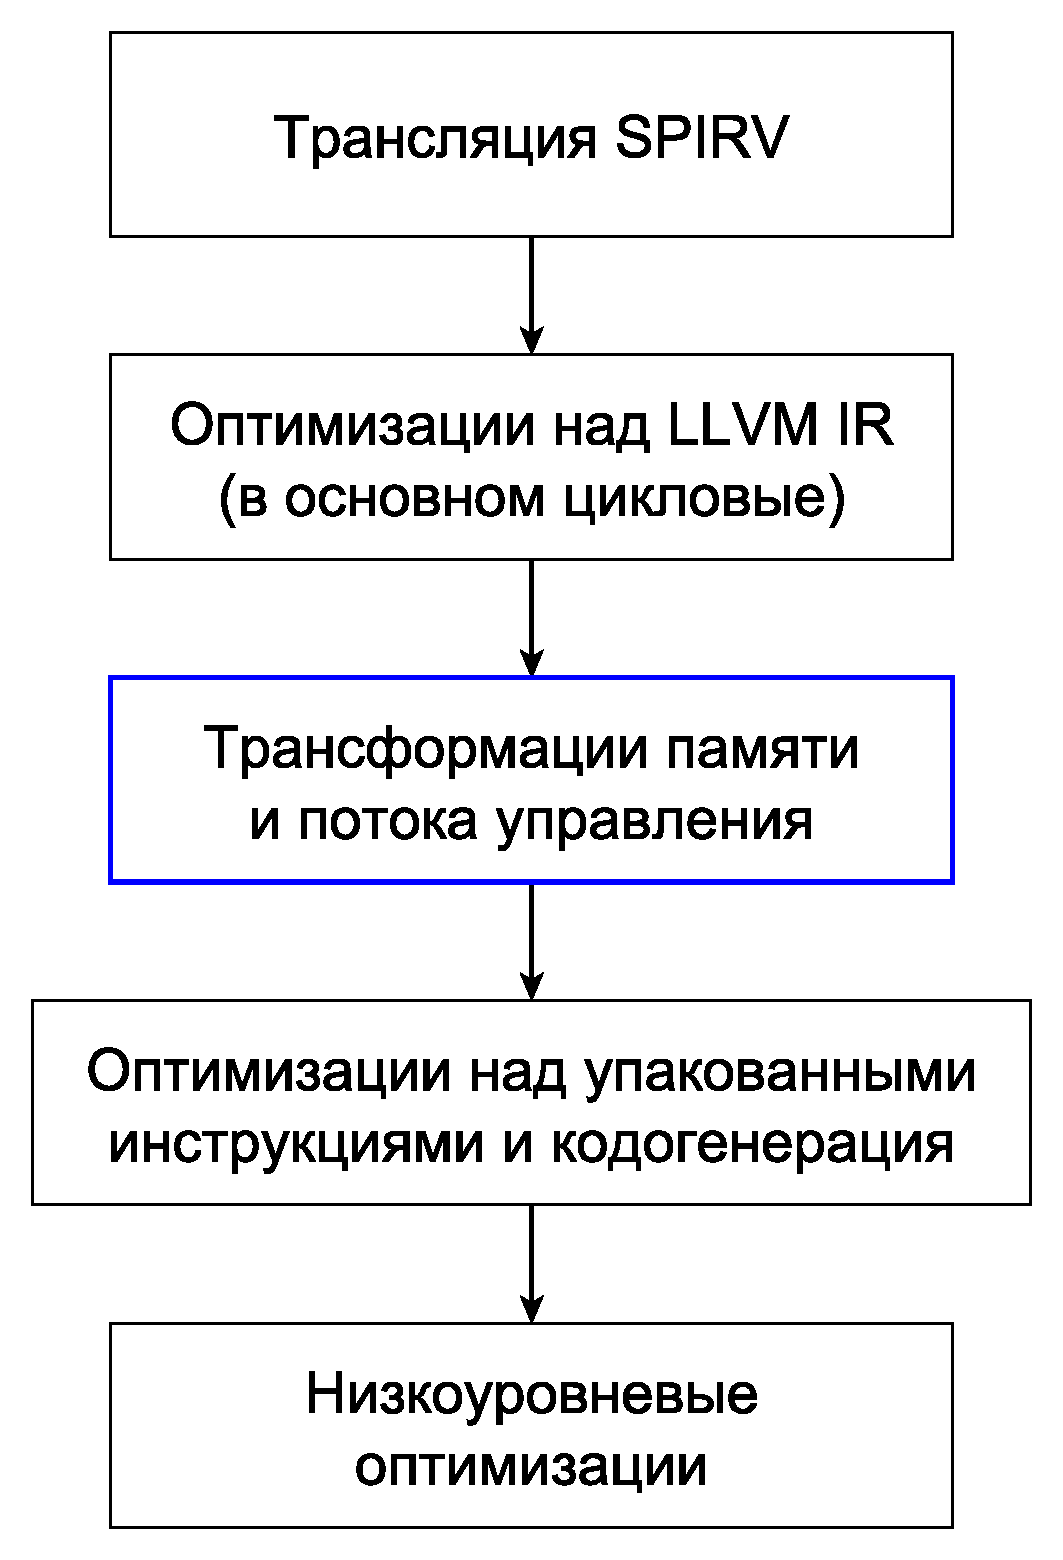
\includegraphics[scale=0.4]{Vladimirov/images/highlevel-mgr.pdf}
    }
    \caption{Высокоуровневый список трансформаций}\label{fig:highlevel-mgr}
\end{figure}

Высокоуровневая схема менеджера пассов представлена на рисунке~\cref{fig:highlevel-mgr}

\begin{figure}[ht]
    \centerfloat{
        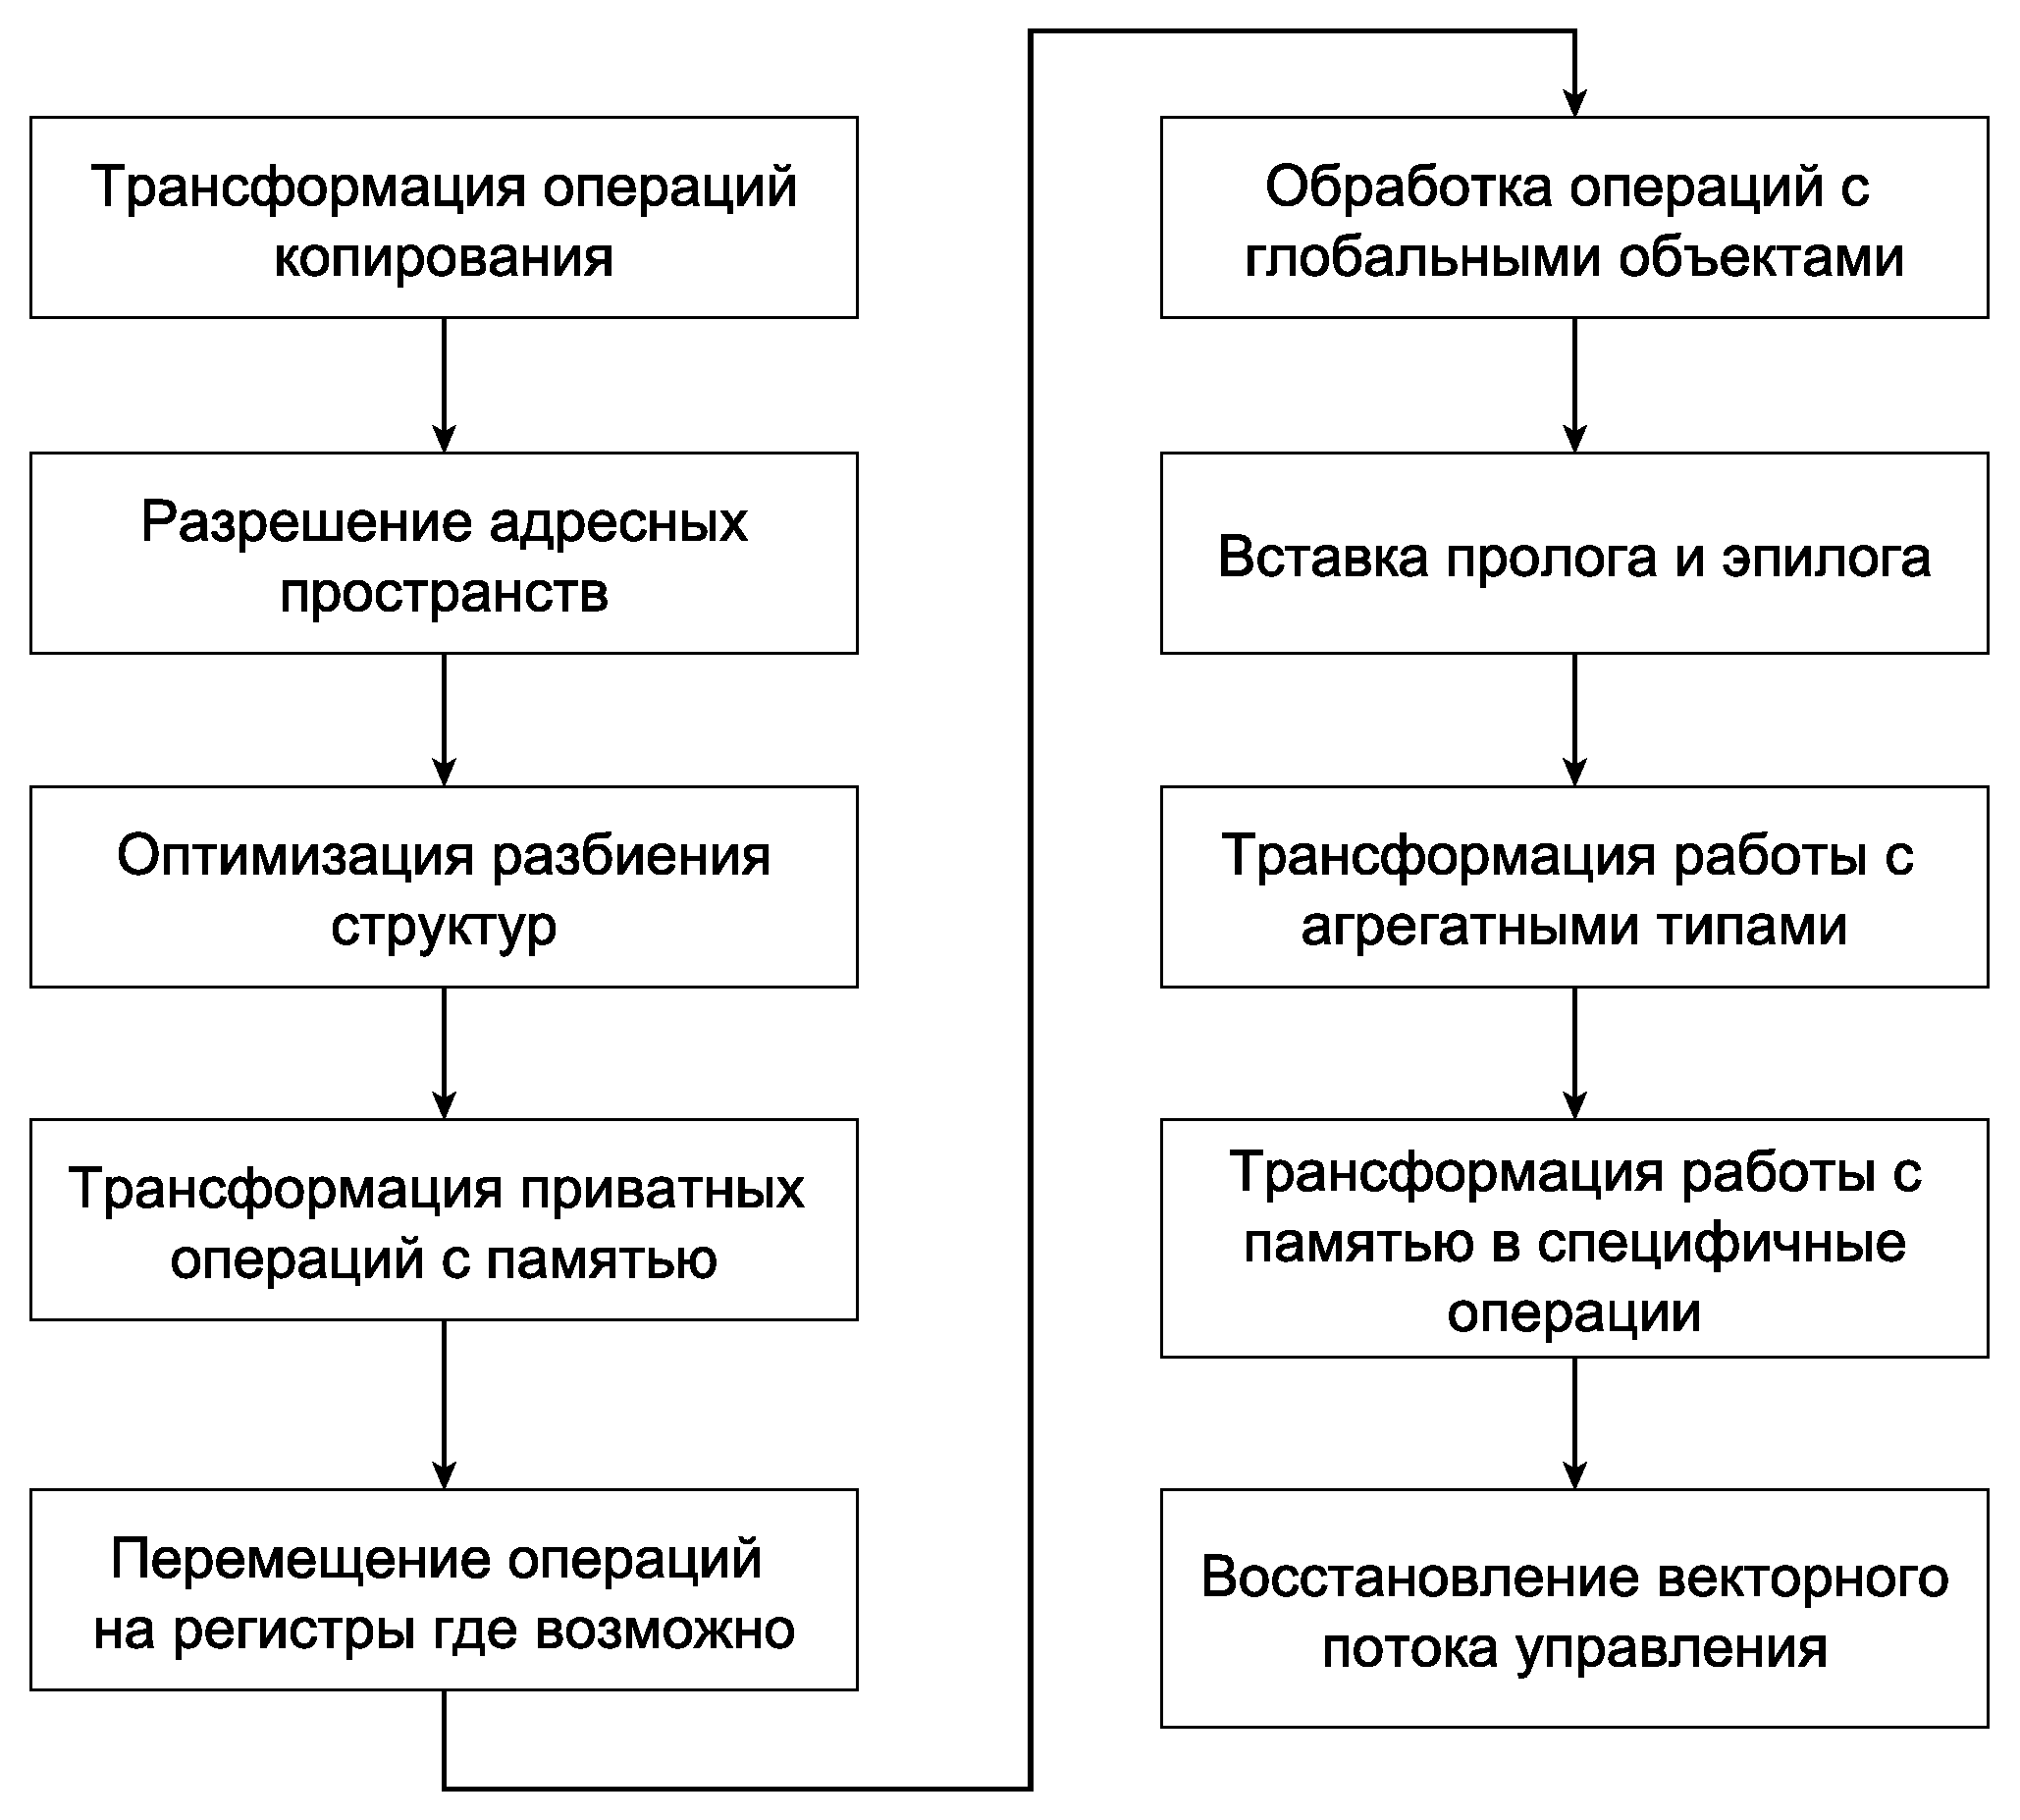
\includegraphics[scale=0.4]{Vladimirov/images/passmgr.pdf}
    }
    \caption{Детальный список трансформаций}\label{fig:passmgr}
\end{figure}

Детальный pass manager представлен на рисунке~\cref{fig:passmgr}

\section{Разбиение структур}\label{sec:lowering/splitter}

Перед описанием алгоритма разбиения определим правила, по которым мы будем выделять части агрегатных типов для векторизации.

В стандарте C++ существует концепция скалярного типа.
Скалярными называются арифметические типы, типы перечислений, указатели и cv-квалифицрованные версии перечисленных типов.
Назовём \emph{базовым} скалярный тип, поддерживаемый данной оптимизацией.
В это множество входят также векторные типы, которых нет в C++, но которые есть в LLVM IR. 
В это множество не входят, например, указатели.
Определение сознательно является несколько нечетким, чтобы заложить возможность будущего расширения.
Алгоритм ниже не разбивает базовые типы.

Назовём \emph{примитивным} либо базовый тип, либо агрегатный тип, у которого типы всех элементов одинаковы и примитивны.
Такой тип нет необходимости делить, так как объекты таких типов могут быть легко переделаны в вектора фазой aggregate lowering, которая представлена в векторном оптимизаторе IGC.
Для алгоритма нет разницы между примитивным типом и базовым, из которого этот примитивный тип состоит, поэтому примитивный всегда будет сводиться к базовому. Например, \verb|< 3 x [ 5 x int]>| будет эквивалентен типу \verb|int|.

Целью алгоритма разбиения структур является приведение всех структур в модуле (например в модуле LLVM IR) к структурам примитивного типа с обязательным сохранением поведения исходной программы в рамках as-if rule.

Фаза разбиения структур в векторном компиляторе разрабатывалась специально для ISPC -- компилятора для SPMD~(single program, multiple data).
При этом алгоритм сам по себе может быть использован в более широких классах оптимизаторов, даже не основанных на LLVM.
Оптимизация работает над LLVM модулем и должна применятся до векторизации.

Разбиение невозможно, если:
\begin{enumerate}
\item элемент структуры является указателем на другую нетривиальную структуру, в том числе на саму себя.
\item на структуру взят указатель.
\end{enumerate}

Первое ограничение появляется из-за использования версии LLVM, в которой ещё не были введены opaque указатели.
Собственноручная поддержка таких указателей приводит к сильному разрастанию получаемого модуля и невозможности применения других оптимизаций.
По этой же причине была невозможна поддержка передачи структур в пользовательские функции.
Второе ограничение связано с тем, что замена кода работы с указателем на аналогичный код с поделёнными структурами может привести к значительному увеличению количества инструкций.

\textbf{Описание алгоритма}

\textbf{Шаг 1. Сбор информации о структурах в модуле}

Информация о структуре хранится в виде хэш-таблицы, где ключ -- это примитивный тип элемента, а значения -- элементы, соответствующие этому типу. Структура в дальнейшем будет делиться как раз по элементам этой хэш-таблицы, так как ключам будет соответствовать примитивный тип, а значениям -- элементы будущей структуры. 
Количество ключей минус один -- столько структур необходимо будет сгенерировать.
Соответственно, если у структуры существует только один примитивный тип, то данную структуру делить нет необходимости, так как она сама является примитивной.

\textbf{Шаг 2. Построение графа вложенности структур}

Так как элементами структуры могут быть другие структуры, то такие ситуации необходимо разрешать.
Граф строится следующим образом: вершине $A$ соответствует структура \%A.
Ребро от вершины $C$ в вершину $A$ проводится в том случае, если структура, соответствующая вершине $A$, вложена в структуру, соответствующую вершине $C$.
Назовём головой графа($Head$) вершины, которые соответствуют структурам, не вложенным ни в какие другие структуры.
Голов графа может быть как одна, так и несколько.

\textbf{Шаг 3. Обработка графа вложенности структур}

Обработка графа начинается с головы, однако деление -- с самой нижней вершины.
Все нижние вершины всегда характеризуются тем, что структуры, связанные с ними содержат элементы только примитивных типов, а значит данные структуры могут быть поделены.
При обработке вершины графа возможны два варианта.
Первое -- если вершина отвечает за примитивную структуру, то в делении нет необходимости и данная вершина удаляется из графа.
Второе -- структура, отвечающая за вершину была поделена.
Тогда нужно заменить во всех структурах, в которые была вложена данная, все элементы, отвечающие за данную структуру, на новые элементы с поделёнными структурами.
Во время замены элементов появляются промежуточные представления структур, которые затем необходимо удалить.
После обработки вершины она удаляется, поэтому все структуры будут обработаны тогда, когда весь граф удалится.

\textbf{Шаг 4. Обработка и замена инструкций}

Обработка инструкций всегда начинается с инструкции выделения памяти на стековом фрейме под структуру (AI -- alloca в LLVM IR).
Далее единственными допустимыми пользователями инструкций выделения памяти являются только инструкции обращения к элементу агрегата (GEP -- getelementptr).
Однако в нашей реализации были допущены инструкции приведения (bitcast) и ptrtoint (PTI) только с определёнными шаблонами использования.
В случае bitcast единственными пользователями могут быть только интринсики lifetime.start/end.
% TODO убрать зависимость от ISPC FE в описании алгоритма
В случае ptrtoint фронтенд ISPC вместо доступа к нулевому элементу структуры через getelementptr использует указатель на структуру.
Данный подход необходимо было поддерживать, поэтому в анализе ptrtoint проверяется соответствие шаблону вычисления указателя из следующих инструкций: insertelement, shufflevector, add и read/write.
В случае если результатом обращения к элементу является примитивный тип, то эта инструкция заменяется на эквивалентную с другим операндом и новой цепочкой индексов.
Если результатом является уже разбитая структура, то будут сгенерированы столько новых обращений, на сколько структур была разбита исходная.

\section{Восстановление векторного потока управления}\label{sec:lowering/simdcf}

TODO: Тут про определение региона

После определения SIMD CF региона можно свести задачу поиска заранее оговоренных конструкций к поиску SIMD CF регионов самого внешнего уровня вложенности, после чего искать вложенные SIMD CF регионы.

Шаг 1. Поиск условного перехода, похожего на векторный поток управления. Для
каждого базового блока проверяется его терминатор. Если это инструкция условного
перехода, то проверяется его условие, в противном случае конструкция не является
SIMD CF регионом. Если условием является результат вызова одного из обозначенных
ранее интринсиков, то идет переход к шагу 2.

Шаг 2. Проверяется структура потока управления и происходит попытка сопоставить
его либо с SIMD CF if/else, либо с SIMD CF циклом. Если сопоставление с одним из
заданных паттернов невозможно, то конструкция не является SIMD CF регионом. В
противном случае происходит переход к шагу 3.

Шаг 3. Проверка маскирования побочных эффектов. Для каждой инструкции, у которой
есть побочные эффекты проводится проверка, является ли такая инструкция
маскирована и если она маскирована, то проверяется, совпадает ли маска для
данной инструкции с условием перехода в эту дугу. Для вложенных регионов
проверяется, является ли маска данного региона подмножеством маски внешнего
региона. Если проверка неудачная - данный регион не является SIMD CF регионом.

Дополнение к шагу 3 для цикла. Проверяются фи-узлы для индуктивностей и пересчет
маски для каждого цикла. Если проверка неудачная - данный регион не является
SIMD CF регионом. В противном случае идет переход к шагу 4.

Дополнение к шагу 3 для if-else. Если кроме if также имеется else, то происходит
проверка, являются ли маски if и else строго противоположны друг другу. Если
проверка неудачная - данный регион не является SIMD CF регионом. В противном
случае идет переход к шагу 4.

Шаг 4. Данный регион является SIMD CF регионом. Аналогично происходит поиск
вложенных SIMD CF регионов для данного региона.

В псевдокоде данный алгоритм будет выглядеть как показано на листинге~\ref{lst:simdcf-analysis}

После сбора всей информации о SIMD CF регионах начинается их оптимизирующая трансформация.

TODO: картинки и трансформация
